\section{Ejercicios propuestos}

\begin{itemize}
    \item Cree una aplicación NodeJS con express, para administrar una agenda personal.
    \item Home (“/”) : Página Principal
    \item Trabaje todo en una misma interfaz.
    \item Ejemplo de estructura de la agenda cuando se explora “Eventos”
    \item La aplicación debe permitir:\newline
	• Crear evento: fecha y hora. (Si ya existe el archivo no debería ingresar el evento)(La primera
	línea es el título del evento, las demás líneas son la descripción del evento. \newline
	• Editar evento. (Se muestran el archivo donde esta el detalle del evento)\newline
	• Eliminar evento.\newline
	• Ver eventos. Utilizar el formato árbol especificado anteriormente, donde debería incluirse
	sólo el título del evento.
\end{itemize}

	
	\subsection*{Cree una aplicación NodeJS con express, para administrar una agenda personal.}

	La elaboracion de la pagina web usando el servidor nodejs y peticiones ajax esta documentado en mi repositorio publico
	que se encuentra en el siguiente enlace: \url{https://github.com/rikich3/pweb2_lab.git}


	\begin{lstlisting}[style=mybash]
		npm init
		npm install express
		npm install --local cors
	\end{lstlisting}
	
	\subsection{Home (“/”) : Página Principal}
	
	Para la mejor separacion de los elementos publicos y carpetas privadas del servidor se esta sirviendo desde una carpeta
	elementos estaticos.

	\begin{lstlisting}[style=js]
		app.use(express.static('pub'));
		\dots
		app.get('/', (request, response)=>{
    	response.sendFile(path.resolve(__dirname, 'pub' , 'index.html'));
		});
	\end{lstlisting}

	El directorio principal termina viendose asi:

	\begin{figure}[h]
		\centering
		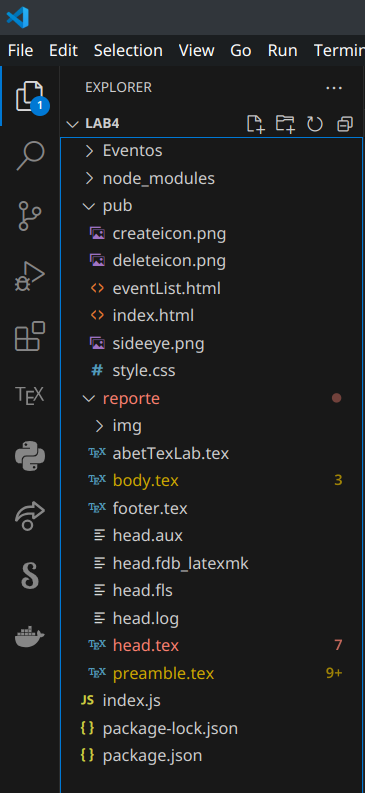
\includegraphics[width=0.3\textwidth]{./img/1.png} % Change example-image to the filename of your image
	\end{figure}


	\subsection{Trabaje todo en una misma interfaz.}

	Toda la aplicacion web estara en una sola pagina web, en index.html adentro de la carpeta pub
	El layout se ve así: 
	\pagebreak
	\begin{figure}[h]
		\centering
		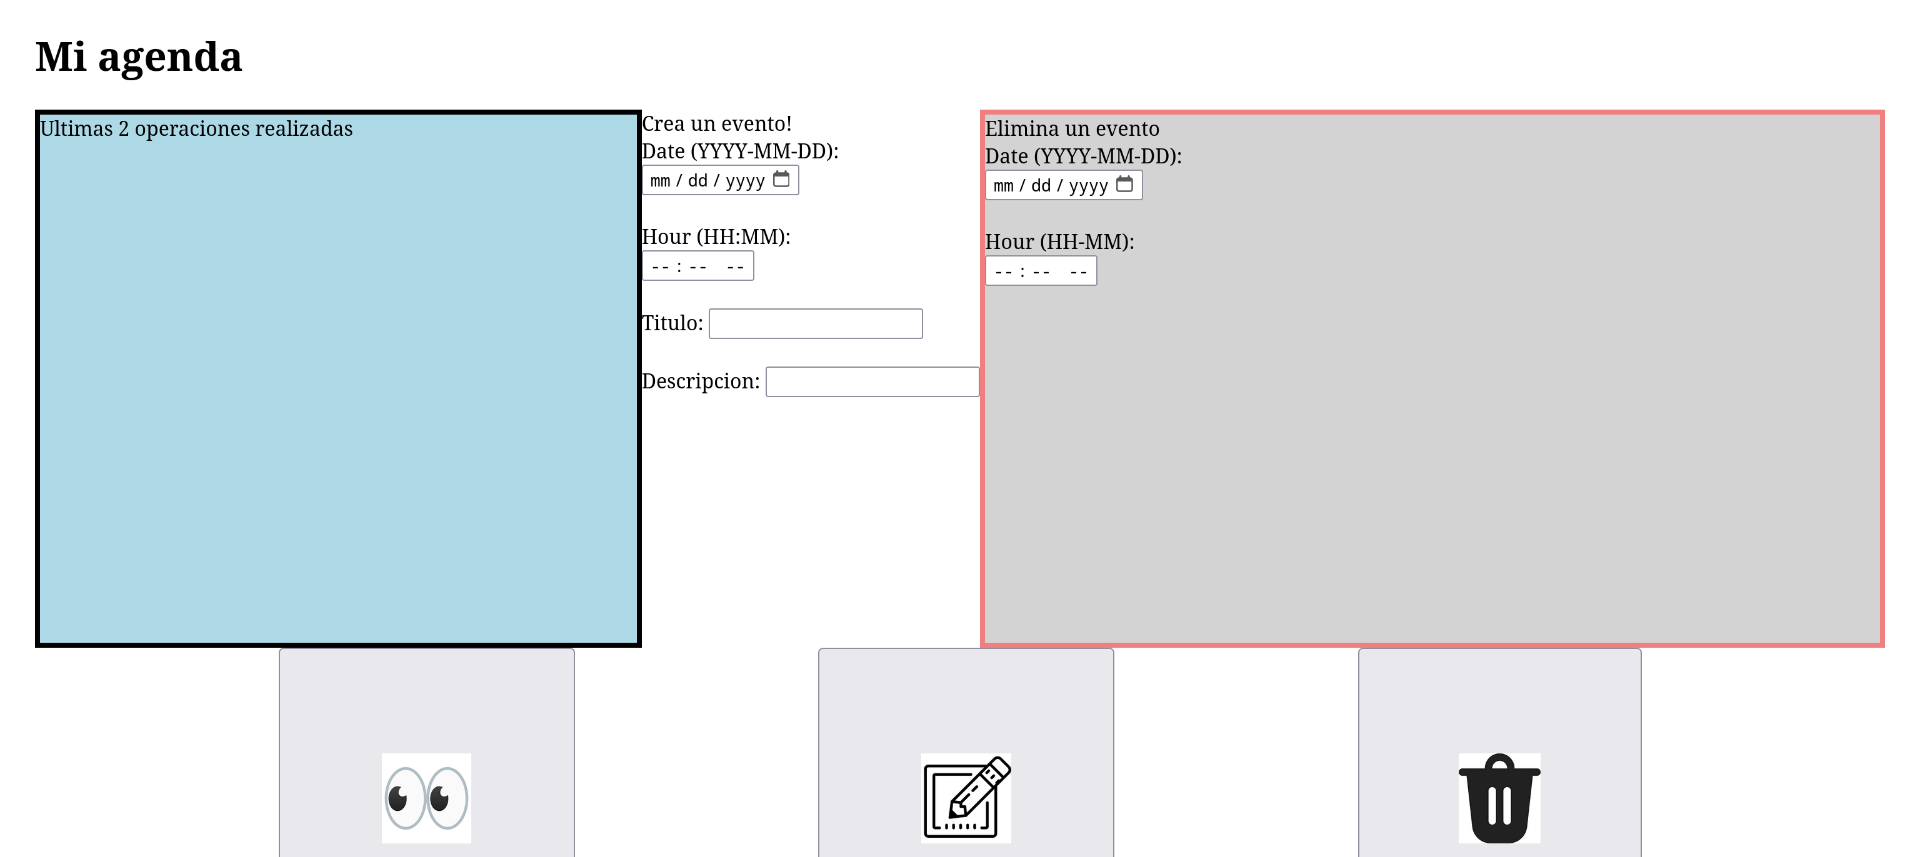
\includegraphics[width=0.9\textwidth]{./img/2.png} % Change example-image to the filename of your image
	\end{figure}
	\newline
	Los forms son para definir los eventos a crear o eliminar y los botones en la parte de abajo para realizar estas acciones.\newline \newline

	
	\subsection{PREGUNTA: Mencione la diferencia entre conexiones asíncronas usando el objeto XmlHttpRequest, JQuery.ajax
	y Fetch. Justifique su respuesta con un ejemplo muy básico. Eje: Hola Mundo, IMC, etc.}

	Fetch API es la opción más moderna y preferida para realizar solicitudes asíncronas en el navegador debido a su sintaxis simple y su uso de promesas. jQuery.ajax() sigue siendo útil en proyectos que ya utilizan jQuery, pero para nuevos proyectos, Fetch API es la opción recomendada. El objeto XHR es la opción más antigua y estándar, pero su uso directo es menos común debido a la disponibilidad de alternativas más modernas y convenientes.
	

\pagebreak